
\documentclass[a4paper, 10pt]{IEEEconf}  

\usepackage{geometry}
\geometry{a4paper, margin=1in}
  
  
\usepackage{subcaption}  
\usepackage[export]{adjustbox}    
\usepackage{verbatim}
\usepackage{graphicx}
\usepackage{pdfpages}
\usepackage{cite}
\usepackage{listings}
\usepackage{float}
\usepackage{url}
\usepackage{hyperref}
\usepackage{fancyhdr}
\usepackage{multicol}

\lstset{
	tabsize=2,
	breaklines=true
}

\setlength{\parskip}{1em}
\onecolumn

\title{\LARGE \bf Assignment 4: Vision-based Automatic Systems\\Industrial Systems Design and Integration 282 772}
\author{Marc Alexander Sferrazza \\ 12164165
\thanks{This work was not supported by any organization}
\thanks{Faculty of Mechatronics Engineering, Massey University, Albany, Auckland, New Zealand
        {\tt\small Progress of project: https://github.com/alex1v1a/Industrial-Systems-Design-and-Integration} } }

\begin{document}

\maketitle
\begin{figure}[H]
  \begin{center}
  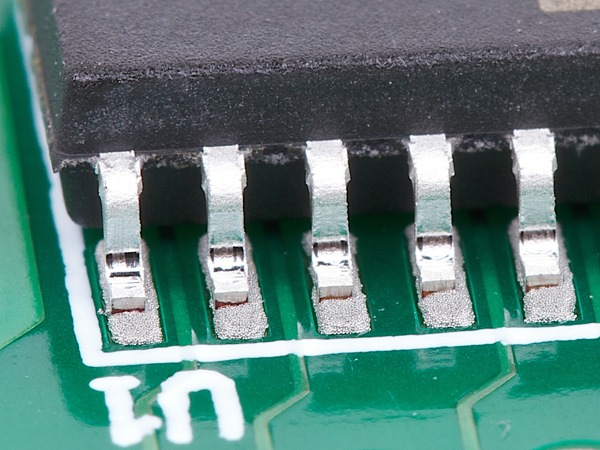
\includegraphics[width=110mm]{images/match}
  \label{fig:kinetic}
  \end{center}
\end{figure}
\thispagestyle{empty}
\pagestyle{plain}


%%%%%%%%%%%%%%%%%%%%%%%%%%%%%%%%%%%%%%%%%%%%%%%%%%%%%%%%%%%%%%%%%%%%%%%%%%%%%%%%

\begin{abstract}
  \begin{center}
	In this documentation, a system is designed with use of OpenCV and TensorFlow that can pick and place electronic Surface Mount Device (SMD) components onto a Printed Circuit Board (PCB) and validate their correct alignment using vision.
  \end{center}
\end{abstract}

%%%%%%%%%%%%%%%%%%%%%%%%%%%%%%%%%%%%%%%%%%%%%%%%%%%%%%%%%%%%%%%%%%%%%%%%%%%%%%%%
%%%%%%%%%%%%%%%%%%%%%%%%%%%%%%%%%%%%%%%%%%%%%%%%%%%%%%%%%%%%%%%%%%%%%%%%%%%%%%%%

\clearpage
\tableofcontents
\listoffigures

%%%%%%%%%%%%%%%%%%%%%%%%%%%%%%%%%%%%%%%%%%%%%%%%%%%%%%%%%%%%%%%%%%%%%%%%%%%%%%%%
%%%%%%%%%%%%%%%%%%%%%%%%%%%%%%%%%%%%%%%%%%%%%%%%%%%%%%%%%%%%%%%%%%%%%%%%%%%%%%%%
\clearpage
\setcounter{page}{1}
%\thispagestyle{empty}
\onecolumn

\section{INTRODUCTION}
Currently there are Automated optical inspection (AOI) devices that scan a PCB with a camera to check alignment and SMT pick and place machines using vision bots to detect orientation and laser coordinate systems. While these current methods are successful and efficient, some of these devices require much fine tuning, and can be difficult to spot the unexpected.

In this task, a system is designed with use of OpenCV that can pick and place electronic Surface Mount Device (SMD) components onto a Printed Circuit Board (PCB) and validate their correct alignment using vision.

%%%%%%%%%%%%%%%%%%%%%%%%%%%%%%%%%%%%%%%%%%%%%%%%%%%%%%%%%%%%%%%%%%%%%%%%%%%%%%%%

\subsection{Aim}
\begin{itemize}
	\item Apply the principles and technologies in intelligent machine design and integration.
	\item Demonstrate familiarity with industrial vision systems and vision-based automatic systems.
\end{itemize}

%%%%%%%%%%%%%%%%%%%%%%%%%%%%%%%%%%%%%%%%%%%%%%%%%%%%%%%%%%%%%%%%%%%%%%%%%%%%%%%%
%\clearpage
\subsection{Machine-vision Algorithm}
%A machine vision algorithm is described and discussed in detail.
An algorithm is used to detect key points and match them. The first stage is to use a cv pointer to and edge detector and an arrow to detect the member function. Multiple images are used with feature mapping to find similar points; using BRISK and ORB for example to find different positions an absolute vector is used $\sqrt(x^2+y^2)$ or another for other types. The function match does the heavy lifting, and will check if this key point matches another current key point and carry on.

While some of these algorithms are fast and available they may not produce perfect results, but while they are not perfect they can be very good in terms of statistical accuracy. Other types of detection algorithms are more restricted e.g. USA based KAZE, SIFT and SURF.

%%%%%%%%%%%%%%%%%%%%%%%%%%%%%%%%%%%%%%%%%%%%%%%%%%%%%%%%%%%%%%%%%%%%%%%%%%%%%%%%
%\clearpage
\subsection{Concepts}
%Several concepts are presented and evaluated using an appropriate quantitative assessment.
Object localisation must fist be used to detect edges, move, transform, and rotate an image, then determine what is relevant and how to ignore outside boundary areas.

With 2D feature detection extractors of key-point descriptors have wrappers so that multiple algorithms can be run on the same images when finding the solution vectors. Not only does it work with both feature detection in a multidimensional space, it also inherits their respective interfaces.

Using feature detection and matching algorithms is the next stage in object localisation. OpenCV has a number of detection tools such as AGAST, GFTT, AKAZE, KAZE, BRISK, MSER, FAST, and ORB. There are also matching algorithms such as BF and FLANN. These algorithms work by finding distinctive points from source images or assigned patterns and compare images.

Using one of these feature detection and matching techniques an object can be localised, transformed and rotated accordingly, then finally matched to the SMD points acquired.

Or using principle component analysis to detect and localise (object localisation) a class that implements everything where the header does the declaration, and cpp does the description. Given enough x and y values with min of 3 values, it can search through randomly to find the points of interest and determine what orientation to look for, show where it is in the image.

%%%%%%%%%%%%%%%%%%%%%%%%%%%%%%%%%%%%%%%%%%%%%%%%%%%%%%%%%%%%%%%%%%%%%%%%%%%%%%%%
%%%%%%%%%%%%%%%%%%%%%%%%%%%%%%%%%%%%%%%%%%%%%%%%%%%%%%%%%%%%%%%%%%%%%%%%%%%%%%%%
\clearpage
\section{CONSTRAINTS} 
%0.5pg
It is important to consider the sensory devices and the effects on the overall system. Due to the limitations of detection equipment choices, common devices used for the information capture are cameras. When using a camera for object orientation detection it is important to notice the lens type, as not all would display a single focal point image capture. When a lens is used image formation geometry can be distorted, therefore a common tool like central perspective imaging may be used to converge a non-inverted image from an image plane. 

To resolve geometric distortion (radial and tangential), spherical aberration, colour fringing and so on; an image can be read in and setting file created, then a rectify map matrix can be used with detorsion coefficients to find and arrange the corrected map.

\begin{figure}[H]
  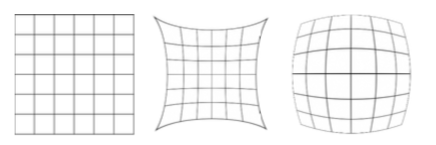
\includegraphics[width=\linewidth,center]{images/lens}
  \caption{Examples of lens distortion, original image, pincushion, and barrel, Image from lecture slide OpenCV 1 \cite{Lecture1}}
  \label{fig:Examples of lens distortion, original image, pincushion, and barrel}
\end{figure}

While cameras are not the only method of image detection delivery, other more object focused methods are offered; however many of these methods may fail on A-semitic components which are more frequent then not.

%%%%%%%%%%%%%%%%%%%%%%%%%%%%%%%%%%%%%%%%%%%%%%%%%%%%%%%%%%%%%%%%%%%%%%%%%%%%%%%%
%\clearpage
\subsection{Environment}
%0.5pg 
Due to such issues caused by time-varying lighting, it is assumed that the environment will be in a production factory, and as such the lighting is kept to an industrial standard; also the image will be read in HSV format not RGB. The advantage of said conditions mean that it is easier to avoid issues and less required compensation can be taken into account for shading areas.

An ideal lens on the camera used for image processing would be a thin convex lens as this has two focus points and is easier to calibrate using central perspective imaging.

Other aspects of hardware may be relevant such as mounting devices and obstructions by such devices, so therefore a good  understanding of these obstructions should be considered and implemented in coding phase. As these are unknown by assumption this section will be excluded from the discussion.

%%%%%%%%%%%%%%%%%%%%%%%%%%%%%%%%%%%%%%%%%%%%%%%%%%%%%%%%%%%%%%%%%%%%%%%%%%%%%%%%
%%%%%%%%%%%%%%%%%%%%%%%%%%%%%%%%%%%%%%%%%%%%%%%%%%%%%%%%%%%%%%%%%%%%%%%%%%%%%%%%
\clearpage
\section{DEVELOPMENTS}
%Several developments are presented and changes described and discussed, and evaluated using an appropriate quantitative assessment.
Using non-homogeneous matrices a retinal plane of coordinates can be found, and when the focus points reach 1 it can be considered normalised. The focus is the first stage as incorrect calibration can result in incorrect matching. 

Feature detection and matching algorithms are used to define not only the shapes of the images but also the orientation of an object. From here if a component were out of alignment, it can be rotated accordingly. 

Object, edge, feature detection, and matching algorithms can also be used to detect an environment. Template matching is somewhat limited, and comparing with sample image and environment space, ignoring some of these aspects that may intrude on the original template can occur in error. For example, if an object were to be rotated, or zoomed out, the template would become somewhat useless or very limited. ORB can deal with rotated and stalled environments, transposed or translated. SIFT and SURF were much slower then ORB and BRISK, but detect more features. AKAZE limits to 500 key points, with more key points detected, the better the object detection, the better the resolution of the object.

%%%%%%%%%%%%%%%%%%%%%%%%%%%%%%%%%%%%%%%%%%%%%%%%%%%%%%%%%%%%%%%%%%%%%%%%%%%%%%%%
%\clearpage
\subsection{Evaluations}

It is in the best interests for this purpose to use the BRISK (and in some cases ORB) for detection with the brute force (BF) matching algorithms, to compute a homography matrix. An image can be localised and external aspects ignored, then after the object detection, features can begin to be examined where matching then takes place. The matching parameters are key in this stage to render key aspects of an object's features as relevant or not, so that if a certain threshold is met it is most likely the same points. The threshold of these values can be sensitive, while too low issues may occur in incorrect matches, and too high can also give false readings if points are found at all and can be a tuning aspect when in play. If a point is found to be correct and within the set threshold it can be considered a good match. 

%%%%%%%%%%%%%%%%%%%%%%%%%%%%%%%%%%%%%%%%%%%%%%%%%%%%%%%%%%%%%%%%%%%%%%%%%%%%%%%%
%\clearpage
\subsection{Final Design}
%A final design is presented and described and discussed in detail.

Object localisation is preformed where corners are examined, key points checked with inspections and scene; brute force is used to produce a homography matrix. After checking both images, and finding the bounding area, the average length of the vectors is checked and a homogenous transform (eg translate) is preformed to locate where it is. After the points on the image are scaled and rotated they are then drawn with the orientation vectors and how much it has been differed from the initial position.

%%%%%%%%%%%%%%%%%%%%%%%%%%%%%%%%%%%%%%%%%%%%%%%%%%%%%%%%%%%%%%%%%%%%%%%%%%%%%%%%
%%%%%%%%%%%%%%%%%%%%%%%%%%%%%%%%%%%%%%%%%%%%%%%%%%%%%%%%%%%%%%%%%%%%%%%%%%%%%%%%
%\clearpage
\section{CRITIQUE}
%1pg
%critical reflection of your design process.
To use object localisation with feature detection and matching, 2 images are needed, the source (camera stream) and desired state. Then by using the BRISK and BF matching the images are read in and do the detection, give the output, adjust and rotate or transform, then wait for the issue to proceed to the next step, align and place the object.

Using brute force and the BRISK matcher, the object is called into play from object localisation where the matcher then goes through each of the descriptors and checks what the max lengths and the minimum lengths were. Then only everything within 60\% of the distances are wanted, otherwise if it is 100\% there will be different points matching wrong places. If the key point is less then 75\% of max distance and greater then 25\% then it's probably correct, not too short and not too long.

The next task is to run through the descriptors and check for good matches; at the end draw the matches, the key points and link them. Adjust the component to those vectors drawn accordingly and begin the loop again. Once no vectors are detected over a certain threshold the object is aligned, so place the object accordingly.

%%%%%%%%%%%%%%%%%%%%%%%%%%%%%%%%%%%%%%%%%%%%%%%%%%%%%%%%%%%%%%%%%%%%%%%%%%%%%%%%
%%%%%%%%%%%%%%%%%%%%%%%%%%%%%%%%%%%%%%%%%%%%%%%%%%%%%%%%%%%%%%%%%%%%%%%%%%%%%%%%

\section{SOLUTIONS}
%1pg
%short description of the machines operation.
%A detailed critical reflection of the employed design process is presented.
Principle component analysis is used to fit a transform matrix to solution vectors, and find how the images have changed, to eventually find the particular orientation of the object. As per the example in the lecture slides using feature matching wrapped inside a class like in the example tutorials e.g. $->$ $feature_match.h$ to declare, and the $feature_match.cpp$ to define the member functions; ORB membership function with the same setup for the key points in first image, and second image for the feature matches using detect and compute, writing a description of those into the descriptive matrix header.
\begin{figure}[H]
  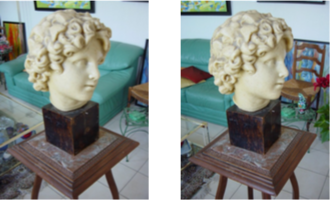
\includegraphics[width=0.7\linewidth,center]{images/1}
  \caption{Original image and orientation, Image from lecture slide OpenCV 2 \cite{Lecture2}}
  \label{fig:Original image and orientation}
\end{figure}
These will result in the object being detected with localisation, then using good matching points as shown below within the threshold.
\begin{figure}[H]
  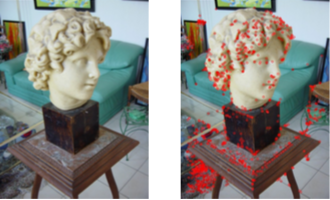
\includegraphics[width=0.7\linewidth,center]{images/2}
  \caption{Good matching points found, Image from lecture slide OpenCV 2 \cite{Lecture2}}
  \label{fig:Good matching points found}
\end{figure}
Once these points are all found the matched points are then conjoined by a red contour. 
\begin{figure}[H]
  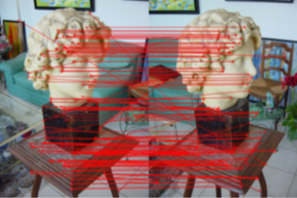
\includegraphics[width=0.7\linewidth,center]{images/3}
  \caption{The final image connecting the good matched points, Image from lecture slide OpenCV 2 \cite{Lecture2}}
  \label{fig:The final image connecting the good matched points}
\end{figure}
The values produced are can be compared to the same for FLANN, just using a CV FLANN matcher rather then a brute force (BF) matcher. There are many different combinations to test run but with the $feature_matcher.h$ $->$ these are the 4 possible combinations BRISK + BF, BRISK + FLANN, ORB + BF, ORB + FLANN

%%%%%%%%%%%%%%%%%%%%%%%%%%%%%%%%%%%%%%%%%%%%%%%%%%%%%%%%%%%%%%%%%%%%%%%%%%%%%%%%
%%%%%%%%%%%%%%%%%%%%%%%%%%%%%%%%%%%%%%%%%%%%%%%%%%%%%%%%%%%%%%%%%%%%%%%%%%%%%%%%

\section{CONCLUSIONS}
A clear knowledge of object localisation is used, and with the application of feature detection and feature mapping algorithms the use of OpenCV camera operations can be performed to successfully align an object while also arranging similar objects and overcoming A-semitic alignment issues. This application however may be unnecessary as current methods suffice, and with reflow soldering most of the components get pulled into place anyway. This application maybe useful for other types of sorting methods however. 

For any progress related to the report please see the public Github repo for alex1v1a or use the link in the cover page to be automatically redirected to this project. The repo provides all relative project information.

NOTE: Please see appendix for sudocode

%%%%%%%%%%%%%%%%%%%%%%%%%%%%%%%%%%%%%%%%%%%%%%%%%%%%%%%%%%%%%%%%%%%%%%%%%%%%%%%%
%%%%%%%%%%%%%%%%%%%%%%%%%%%%%%%%%%%%%%%%%%%%%%%%%%%%%%%%%%%%%%%%%%%%%%%%%%%%%%%%

\clearpage
\nocite{*}
\bibliographystyle{ieeetr}
\bibliography{references}

%%%%%%%%%%%%%%%%%%%%%%%%%%%%%%%%%%%%%%%%%%%%%%%%%%%%%%%%%%%%%%%%%%%%%%%%%%%%%%%%
%%%%%%%%%%%%%%%%%%%%%%%%%%%%%%%%%%%%%%%%%%%%%%%%%%%%%%%%%%%%%%%%%%%%%%%%%%%%%%%%

%\clearpage
\onecolumn
\section*{APPENDIX}
\begin{lstlisting}[language = c++]
object pca

#includes

init camera

rectify map matrix (dist K, map org, map correct)

objectlocalizer()

const bool object localiser::ORBorBRISK(const cv::Mat ... map config)
	
	ORBorBRISK create
	loop for transforms{
		detect and compute
	
		switch(matcher){
			brute force or FLANN
			vector matching
			
			loop for descriptors(rows.. ++){
				dist = matches..
				if (dist < min) min = dist
				if (dist > max) mac = dist
			
				-- Out of threshold max ranges
			}
			loop through matches {
				check threshold range opti
			}
			send back good matches
		
			draw links to each point
		
			connected all vectors
		
			contours, bounding, corners, bounding rect etc...
		
			return vector arrange dist
		}
		ADS 
		Port...
	
		Pick up request... 
		PLC
		state high state low on axis ports to transform degrees of freedom
	
		Rotate and transform according to vectors
		check vector threshold if under lim then finish
	}
	cleanup...
	destroy all win
	break	
etc
\end{lstlisting}

\end{document}